\documentclass{beamer}

\usetheme{default}

\definecolor{ufabcblue}{RGB}{0,51,153}
\definecolor{lightgray}{RGB}{240,240,240}
\usepackage{graphicx}
\usepackage{booktabs}
\usepackage[normalem]{ulem} % para taxar os textos
\usepackage{xcolor}

\setbeamertemplate{navigation symbols}{}

\setbeamercolor{background canvas}{bg=white}

\setbeamercolor{title}{fg=ufabcblue}
\setbeamerfont{title}{series=\bfseries, size=\Large}
\setbeamercolor{structure}{fg=ufabcblue}

\setbeamertemplate{footline}{
  \leavevmode
  \hbox{
    \begin{beamercolorbox}[wd=.33\paperwidth,ht=2.5ex,dp=1ex,center]{author in head/foot}
      \color{white}\scriptsize William Fernandes Dias
    \end{beamercolorbox}
    \begin{beamercolorbox}[wd=.34\paperwidth,ht=2.5ex,dp=1ex,center]{title in head/foot}
      \color{white}\scriptsize UFABC/CMCC
    \end{beamercolorbox}
    \begin{beamercolorbox}[wd=.33\paperwidth,ht=2.5ex,dp=1ex,center]{date in head/foot}
      \color{white}\scriptsize \insertshortdate \hspace{1em} \insertframenumber/\inserttotalframenumber
    \end{beamercolorbox}
  }
}

\setbeamercolor{author in head/foot}{bg=ufabcblue}
\setbeamercolor{title in head/foot}{bg=ufabcblue}
\setbeamercolor{date in head/foot}{bg=ufabcblue}

\title{Comparativo de Estratégias para Lidar com Desbalanceamento de Dados na Avaliação de Risco de Crédito}

\author{William Fernandes Dias\\
Orientador: Dr. Paulo Henrique Pisani}

\institute{Universidade Federal do ABC\\
  Centro de Matemática, Computação e Cognição\\
Projeto de Graduação em Computação}

\date{23 de abril de 2026}

\setbeamertemplate{itemize item}{\textbullet}
\setbeamertemplate{itemize subitem}{\textbullet}
\setbeamertemplate{itemize subsubitem}{\textbullet}

\setbeamertemplate{frametitle continuation}{}

\begin{document}

% Slide de capa
\begin{frame}
  \titlepage
\end{frame}

% Slide padrão
\begin{frame}{Organização da apresentação}
  \begin{itemize}
    \item Introdução
    \item Objetivos
    \item Metodologia
      \begin{itemize}
        \item Conjuntos de dados
        \item Modelos de aprendizado de máquina
        \item Estratégias para lidar com desbalanceamento de dados
        \item Métricas de desempenho
        \item Experimentos
      \end{itemize}
    \item Resultados
      \begin{itemize}
        \item Métricas de desempenho
        \item Desempenho Custo-sensível vs Re-amostragem
        \item \textit{Trade-off} entre Precisão e Sensibilidade
      \end{itemize}
    \item Discussão
    \item Conclusão e trabalhos futuros
  \end{itemize}
\end{frame}

\begin{frame}{Introdução}
  \begin{itemize}
    \item[$\blacktriangleright$] Risco de crédito.
      \begin{itemize}
        \item Processo de avaliação da probabilidade de inadimplência de um cliente.
        \item É essencial para a manutenção da estabilidade, rentabilidade e confiança nas operações das instituições financeiras.
        \item Falhas sistêmicas nesta avaliação podem desencadear crises em escala global
          \begin{itemize}
            \item[Exemplo:] Crise imobiliária de 2008~\cite{Christiano2008}
          \end{itemize}
      \end{itemize}
  \end{itemize}
\end{frame}

\begin{frame}{Introdução}
  \begin{itemize}
    \item[$\blacktriangleright$] Aprendizado de máquina
      \begin{itemize}
        \item Tradicionalmente dependentes de modelos estatísticos subjetivos e suscetíveis a vieses humanos.
        \item A adoção de modelos de Aprendizado de Máquina surge como alternativa superior, permitindo a identificação de padrões complexos~\cite{Shi2022}.
        \item[Problema:] Desbalanceamento de dados
          \begin{itemize}
            \item A maioria dos clientes é adimplente, o que pode levar a modelos tendenciosos e ineficazes~\cite{Namvar2018}.
          \end{itemize}
      \end{itemize}
  \end{itemize}
\end{frame}

\begin{frame}{Objetivos}
  \begin{itemize}
    \item[$\blacktriangleright$] Objetivo geral
      \begin{itemize}
        \item Avaliar o desempenho de diferentes estratégias para lidar com o desbalanceamento de dados na avaliação de risco de crédito.
      \end{itemize}
    \item[$\blacktriangleright$] Objetivos específicos
      \begin{itemize}
        \item Comparar o desempenho de modelos de aprendizado de máquina treinados com e sem estratégias de balanceamento.
        \item Analisar a eficácia de diferentes técnicas de balanceamento, como \textit{oversampling}, \textit{under-sampling} e algoritmos específicos para dados desbalanceados em diferentes contextos de crédito.
      \end{itemize}
  \end{itemize}
\end{frame}

\begin{frame}{Metodologia}
  \begin{itemize}
    \item[$\blacktriangleright$] Conjuntos de dados
  \end{itemize}

  \vspace{-0.4em}
  \footnotesize
  \setlength{\tabcolsep}{3pt}
  \renewcommand{\arraystretch}{1.15}

  \begin{table}[h]
    \centering
    \begin{tabular}{|l|c|c|c|}
      \hline
      \textbf{Indicador} & \textbf{Lending Club} & \textbf{Taiwan} & \textbf{Corporate Credit} \\
      \hline
      Origem/Tipo & P2P (EUA) & Cartões (PF) & Empresas \\
      \hline
      Amostras & 630 mil & 30 mil & 2.029 \\
      \hline
      Atributos & 145 & 24 & 31 \\
      \hline
      Inadimplentes & 1,1\% & 22\% & 2,8\% \\
      \hline
    \end{tabular}
  \end{table}
  \normalsize
\end{frame}

\begin{frame}{Metodologia}
  \begin{itemize}
    \item[$\blacktriangleright$] Modelos de aprendizado de máquina
      \begin{itemize}
        \item SVM
        \item Random Forest
        \item XGBoost
        \item MLP
      \end{itemize}
  \end{itemize}
\end{frame}

\begin{frame}{Metodologia}
  \begin{itemize}
    \item[$\blacktriangleright$] Estratégias para lidar com desbalanceamento de dados
      \begin{itemize}
        \item SMOTE (oversampling)
        \item RUS (under-sampling)
        \item SMOTE-Tomek (híbrido)
        \item CS-SVM (sensível a custos)
      \end{itemize}
  \end{itemize}
\end{frame}

\begin{frame}{Metodologia}
  \begin{itemize}
    \item[$\blacktriangleright$] Métricas de desempenho
      \begin{itemize}
        \item Acurácia balanceada
        \item F1-score
        \item G-mean
        \item Precisão
        \item Sensibilidade
      \end{itemize}
  \end{itemize}
\end{frame}

\begin{frame}{Metodologia}
  \begin{itemize}
    \item[$\blacktriangleright$] Experimentos
      \begin{itemize}
        \item Validação cruzada estratificada
        \item Separação dos dados em conjuntos de treinamento e teste
          \begin{itemize}
            \item Treinamento: 70\%
            \item Teste: 30\%
          \end{itemize}
        \item Busca em grade para otimização de hiper-parâmetros
        \item Média de 5 sementes para cada combinação de modelo e estratégia, totalizando 85 experimentos por conjunto de dados.
      \end{itemize}
  \end{itemize}
\end{frame}

\begin{frame}{Resultados}

  \begin{itemize}
    \item[$\blacktriangleright$] Métricas de desempenho
      \begin{itemize}
        \item Lending Club
      \end{itemize}
  \end{itemize}

  \scriptsize
  \setlength{\tabcolsep}{2pt}
  \renewcommand{\arraystretch}{1.05}

  \begin{table}[h]
    \centering
    \resizebox{\textwidth}{!}{%
      \begin{tabular}{|l|l|c|c|c|c|c|c|}
        \hline
        \textbf{Modelo} & \textbf{Técnica} & \textbf{Acur. Bal.} & \textbf{G-Mean} & \textbf{F1} & \textbf{Precisão} & \textbf{Sensib.} & \textbf{Especif.} \\
        \hline
        XGBoost & RUS & 0.6590 (0.0005) & 0.6589 (0.0005) & 0.4352 (0.0006) & 0.3237 (0.0007) & 0.6639 (0.0021) & 0.6541 (0.0019) \\
        \hline
        MLP & RUS & 0.6588 (0.0008) & 0.6582 (0.0010) & 0.4344 (0.0019) & 0.3203 (0.0074) & 0.6758 (0.0237) & 0.6418 (0.0244) \\
        \hline
        Random Forest & RUS & 0.6506 (0.0006) & 0.6506 (0.0006) & 0.4266 (0.0006) & 0.3181 (0.0006) & 0.6472 (0.0020) & 0.6539 (0.0016) \\
        \hline
        SVM & CS-SVM & 0.6466 (0.0005) & 0.6464 (0.0006) & 0.4228 (0.0004) & 0.3179 (0.0013) & 0.6312 (0.0056) & 0.6621 (0.0049) \\
        \hline
        SVM & RUS & 0.6465 (0.0004) & 0.6461 (0.0006) & 0.4229 (0.0002) & 0.3194 (0.0020) & 0.6254 (0.0081) & 0.6676 (0.0074) \\
        \hline
        SVM & SMOTE-Tomek & 0.6462 (0.0005) & 0.6461 (0.0005) & 0.4222 (0.0005) & 0.3165 (0.0010) & 0.6341 (0.0032) & 0.6584 (0.0032) \\
        \hline
        SVM & SMOTE & 0.6461 (0.0003) & 0.6460 (0.0003) & 0.4221 (0.0004) & 0.3167 (0.0011) & 0.6329 (0.0038) & 0.6594 (0.0037) \\
        \hline
        Random Forest & SMOTE & 0.6237 (0.0009) & 0.6118 (0.0054) & 0.3980 (0.0012) & 0.3291 (0.0124) & 0.5060 (0.0295) & 0.7414 (0.0298) \\
        \hline
        Random Forest & SMOTE-Tomek & 0.6235 (0.0009) & 0.6130 (0.0049) & 0.3978 (0.0011) & 0.3257 (0.0121) & 0.5131 (0.0277) & 0.7338 (0.0286) \\
        \hline
        MLP & SMOTE & 0.6231 (0.0082) & 0.6029 (0.0149) & 0.3967 (0.0112) & 0.3451 (0.0056) & 0.4680 (0.0349) & 0.7783 (0.0200) \\
        \hline
        XGBoost & SMOTE & 0.6157 (0.0015) & 0.5944 (0.0032) & 0.3870 (0.0021) & 0.3366 (0.0012) & 0.4553 (0.0080) & 0.7761 (0.0051) \\
        \hline
        MLP & SMOTE-Tomek & 0.6041 (0.0039) & 0.5618 (0.0118) & 0.3674 (0.0071) & 0.3540 (0.0075) & 0.3829 (0.0242) & 0.8254 (0.0168) \\
        \hline
        XGBoost & SMOTE-Tomek & 0.5618 (0.0006) & 0.4041 (0.0022) & 0.2516 (0.0019) & 0.4719 (0.0028) & 0.1715 (0.0020) & 0.9521 (0.0009) \\
        \hline
        XGBoost & Linha de Base & 0.5422 (0.0008) & 0.3239 (0.0021) & 0.1791 (0.0022) & 0.5387 (0.0049) & 0.1074 (0.0014) & 0.9771 (0.0002) \\
        \hline
        MLP & Linha de Base & 0.5348 (0.0016) & 0.2911 (0.0067) & 0.1496 (0.0060) & 0.5639 (0.0037) & 0.0862 (0.0040) & 0.9834 (0.0009) \\
        \hline
        SVM & Linha de Base & 0.5306 (0.0041) & 0.2780 (0.0188) & 0.1371 (0.0164) & 0.5277 (0.0067) & 0.0790 (0.0110) & 0.9823 (0.0029) \\
        \hline
        Random Forest & Linha de Base & 0.5212 (0.0004) & 0.2270 (0.0022) & 0.0954 (0.0017) & 0.5748 (0.0051) & 0.0520 (0.0010) & 0.9904 (0.0003) \\
        \hline
      \end{tabular}%
    }
  \end{table}
  \normalsize
\end{frame}

\begin{frame}{Resultados}

  \begin{itemize}
    \item[$\blacktriangleright$] Métricas de desempenho
      \begin{itemize}
        \item Taiwan Credit
      \end{itemize}
  \end{itemize}

  \scriptsize
  \setlength{\tabcolsep}{2pt}
  \renewcommand{\arraystretch}{1.05}

  \begin{table}[h]
    \centering
    \resizebox{\textwidth}{!}{%
      \begin{tabular}{|l|l|c|c|c|c|c|c|}
        \hline
        \textbf{Modelo} & \textbf{Técnica} & \textbf{Acur. Bal.} & \textbf{G-Mean} & \textbf{F1} & \textbf{Precisão} & \textbf{Sensib.} & \textbf{Especif.} \\
        \hline
        XGBoost & RUS & 0.7108 (0.0058) & 0.7065 (0.0069) & 0.5324 (0.0076) & 0.4592 (0.0122) & 0.6342 (0.0181) & 0.7874 (0.0139) \\
        \hline
        Random Forest & RUS & 0.7106 (0.0058) & 0.7036 (0.0070) & 0.5359 (0.0079) & 0.4769 (0.0135) & 0.6123 (0.0175) & 0.8088 (0.0136) \\
        \hline
        Random Forest & SMOTE & 0.7067 (0.0051) & 0.6947 (0.0057) & 0.5360 (0.0075) & 0.5006 (0.0092) & 0.5770 (0.0091) & 0.8364 (0.0058) \\
        \hline
        Random Forest & SMOTE-Tomek & 0.7065 (0.0052) & 0.6945 (0.0058) & 0.5356 (0.0077) & 0.4996 (0.0096) & 0.5773 (0.0092) & 0.8357 (0.0060) \\
        \hline
        MLP & RUS & 0.7033 (0.0051) & 0.6952 (0.0071) & 0.5263 (0.0053) & 0.4702 (0.0068) & 0.5981 (0.0198) & 0.8084 (0.0109) \\
        \hline
        XGBoost & SMOTE-Tomek & 0.7020 (0.0051) & 0.6891 (0.0058) & 0.5296 (0.0077) & 0.4962 (0.0111) & 0.5680 (0.0103) & 0.8360 (0.0079) \\
        \hline
        XGBoost & SMOTE & 0.7016 (0.0051) & 0.6885 (0.0059) & 0.5291 (0.0074) & 0.4963 (0.0092) & 0.5667 (0.0101) & 0.8365 (0.0062) \\
        \hline
        SVM & CS-SVM & 0.7011 (0.0046) & 0.6870 (0.0061) & 0.5291 (0.0059) & 0.5003 (0.0021) & 0.5615 (0.0117) & 0.8407 (0.0029) \\
        \hline
        MLP & SMOTE-Tomek & 0.7010 (0.0049) & 0.6970 (0.0044) & 0.5186 (0.0087) & 0.4425 (0.0208) & 0.6278 (0.0193) & 0.7743 (0.0242) \\
        \hline
        SVM & SMOTE & 0.7002 (0.0056) & 0.6862 (0.0080) & 0.5276 (0.0072) & 0.4979 (0.0070) & 0.5614 (0.0168) & 0.8391 (0.0078) \\
        \hline
        SVM & SMOTE-Tomek & 0.6998 (0.0040) & 0.6849 (0.0059) & 0.5277 (0.0049) & 0.5018 (0.0018) & 0.5565 (0.0122) & 0.8430 (0.0043) \\
        \hline
        SVM & RUS & 0.6976 (0.0031) & 0.6833 (0.0052) & 0.5237 (0.0037) & 0.4943 (0.0080) & 0.5573 (0.0134) & 0.8379 (0.0086) \\
        \hline
        MLP & SMOTE & 0.6974 (0.0066) & 0.6923 (0.0065) & 0.5147 (0.0103) & 0.4431 (0.0200) & 0.6155 (0.0208) & 0.7793 (0.0237) \\
        \hline
        XGBoost & Linha de Base & 0.6579 (0.0049) & 0.5902 (0.0082) & 0.4743 (0.0096) & 0.6695 (0.0137) & 0.3673 (0.0106) & 0.9484 (0.0034) \\
        \hline
        MLP & Linha de Base & 0.6572 (0.0092) & 0.5908 (0.0175) & 0.4723 (0.0179) & 0.6554 (0.0161) & 0.3699 (0.0237) & 0.9446 (0.0066) \\
        \hline
        Random Forest & Linha de Base & 0.6552 (0.0053) & 0.5862 (0.0089) & 0.4689 (0.0105) & 0.6634 (0.0124) & 0.3627 (0.0113) & 0.9477 (0.0030) \\
        \hline
        SVM & Linha de Base & 0.6240 (0.0365) & 0.5216 (0.0778) & 0.3971 (0.0851) & 0.6636 (0.0359) & 0.2901 (0.0870) & 0.9579 (0.0156) \\
        \hline
      \end{tabular}%
    }
  \end{table}
  \normalsize
\end{frame}

\begin{frame}{Resultados}

  \begin{itemize}
    \item[$\blacktriangleright$] Métricas de desempenho
      \begin{itemize}
        \item Corporate Credit Rating
      \end{itemize}
  \end{itemize}

  \scriptsize
  \setlength{\tabcolsep}{2pt}
  \renewcommand{\arraystretch}{1.05}

  \begin{table}[h]
    \centering
    \resizebox{\textwidth}{!}{%
      \begin{tabular}{|l|l|c|c|c|c|c|c|}
        \hline
        \textbf{Modelo} & \textbf{Técnica} & \textbf{Acur. Bal.} & \textbf{G-Mean} & \textbf{F1} & \textbf{Precisão} & \textbf{Sensib.} & \textbf{Especif.} \\
        \hline
        MLP & SMOTE & 0.8274 (0.1336) & 0.8050 (0.1537) & 0.0935 (0.0275) & 0.0505 (0.0152) & 0.7000 (0.2739) & 0.9549 (0.0151) \\
        \hline
        MLP & SMOTE-Tomek & 0.8274 (0.1336) & 0.8050 (0.1537) & 0.0935 (0.0275) & 0.0505 (0.0152) & 0.7000 (0.2739) & 0.9549 (0.0151) \\
        \hline
        SVM & RUS & 0.7680 (0.1238) & 0.7536 (0.1240) & 0.0209 (0.0069) & 0.0106 (0.0036) & 0.8000 (0.2739) & 0.7361 (0.0889) \\
        \hline
        MLP & RUS & 0.7263 (0.1258) & 0.7090 (0.1284) & 0.0211 (0.0115) & 0.0108 (0.0059) & 0.7000 (0.2739) & 0.7526 (0.1256) \\
        \hline
        Random Forest & RUS & 0.6217 (0.1323) & 0.4104 (0.3747) & 0.0317 (0.0327) & 0.0168 (0.0176) & 0.3000 (0.2739) & 0.9433 (0.0261) \\
        \hline
        SVM & CS-SVM & 0.6156 (0.1318) & 0.4071 (0.3718) & 0.0305 (0.0371) & 0.0163 (0.0204) & 0.3000 (0.2739) & 0.9311 (0.0467) \\
        \hline
        XGBoost & RUS & 0.6013 (0.2175) & 0.4355 (0.4041) & 0.0167 (0.0166) & 0.0086 (0.0086) & 0.4000 (0.4183) & 0.8026 (0.1276) \\
        \hline
        SVM & SMOTE & 0.5839 (0.1350) & 0.2775 (0.3801) & 0.0413 (0.0669) & 0.0237 (0.0394) & 0.2000 (0.2739) & 0.9677 (0.0161) \\
        \hline
        SVM & SMOTE-Tomek & 0.5839 (0.1350) & 0.2775 (0.3801) & 0.0413 (0.0669) & 0.0237 (0.0394) & 0.2000 (0.2739) & 0.9677 (0.0161) \\
        \hline
        MLP & Linha de Base & 0.5449 (0.1091) & 0.1400 (0.3131) & 0.0267 (0.0596) & 0.0154 (0.0344) & 0.1000 (0.2236) & 0.9898 (0.0055) \\
        \hline
        Random Forest & Linha de Base & 0.5000 (0.0000) & 0.0000 (0.0000) & 0.0000 (0.0000) & 0.0000 (0.0000) & 0.0000 (0.0000) & 1.0000 (0.0000) \\
        \hline
        XGBoost & Linha de Base & 0.5000 (0.0000) & 0.0000 (0.0000) & 0.0000 (0.0000) & 0.0000 (0.0000) & 0.0000 (0.0000) & 1.0000 (0.0000) \\
        \hline
        SVM & Linha de Base & 0.4990 (0.0015) & 0.0000 (0.0000) & 0.0000 (0.0000) & 0.0000 (0.0000) & 0.0000 (0.0000) & 0.9980 (0.0029) \\
        \hline
        Random Forest & SMOTE-Tomek & 0.4985 (0.0014) & 0.0000 (0.0000) & 0.0000 (0.0000) & 0.0000 (0.0000) & 0.0000 (0.0000) & 0.9970 (0.0027) \\
        \hline
        Random Forest & SMOTE & 0.4985 (0.0014) & 0.0000 (0.0000) & 0.0000 (0.0000) & 0.0000 (0.0000) & 0.0000 (0.0000) & 0.9970 (0.0027) \\
        \hline
        XGBoost & SMOTE-Tomek & 0.4934 (0.0065) & 0.0000 (0.0000) & 0.0000 (0.0000) & 0.0000 (0.0000) & 0.0000 (0.0000) & 0.9868 (0.0129) \\
        \hline
        XGBoost & SMOTE & 0.4934 (0.0065) & 0.0000 (0.0000) & 0.0000 (0.0000) & 0.0000 (0.0000) & 0.0000 (0.0000) & 0.9868 (0.0129) \\
        \hline
      \end{tabular}%
    }
  \end{table}
  \normalsize
\end{frame}

\begin{frame}{Resultados}
  \vspace{-0.4em}
  \centering
  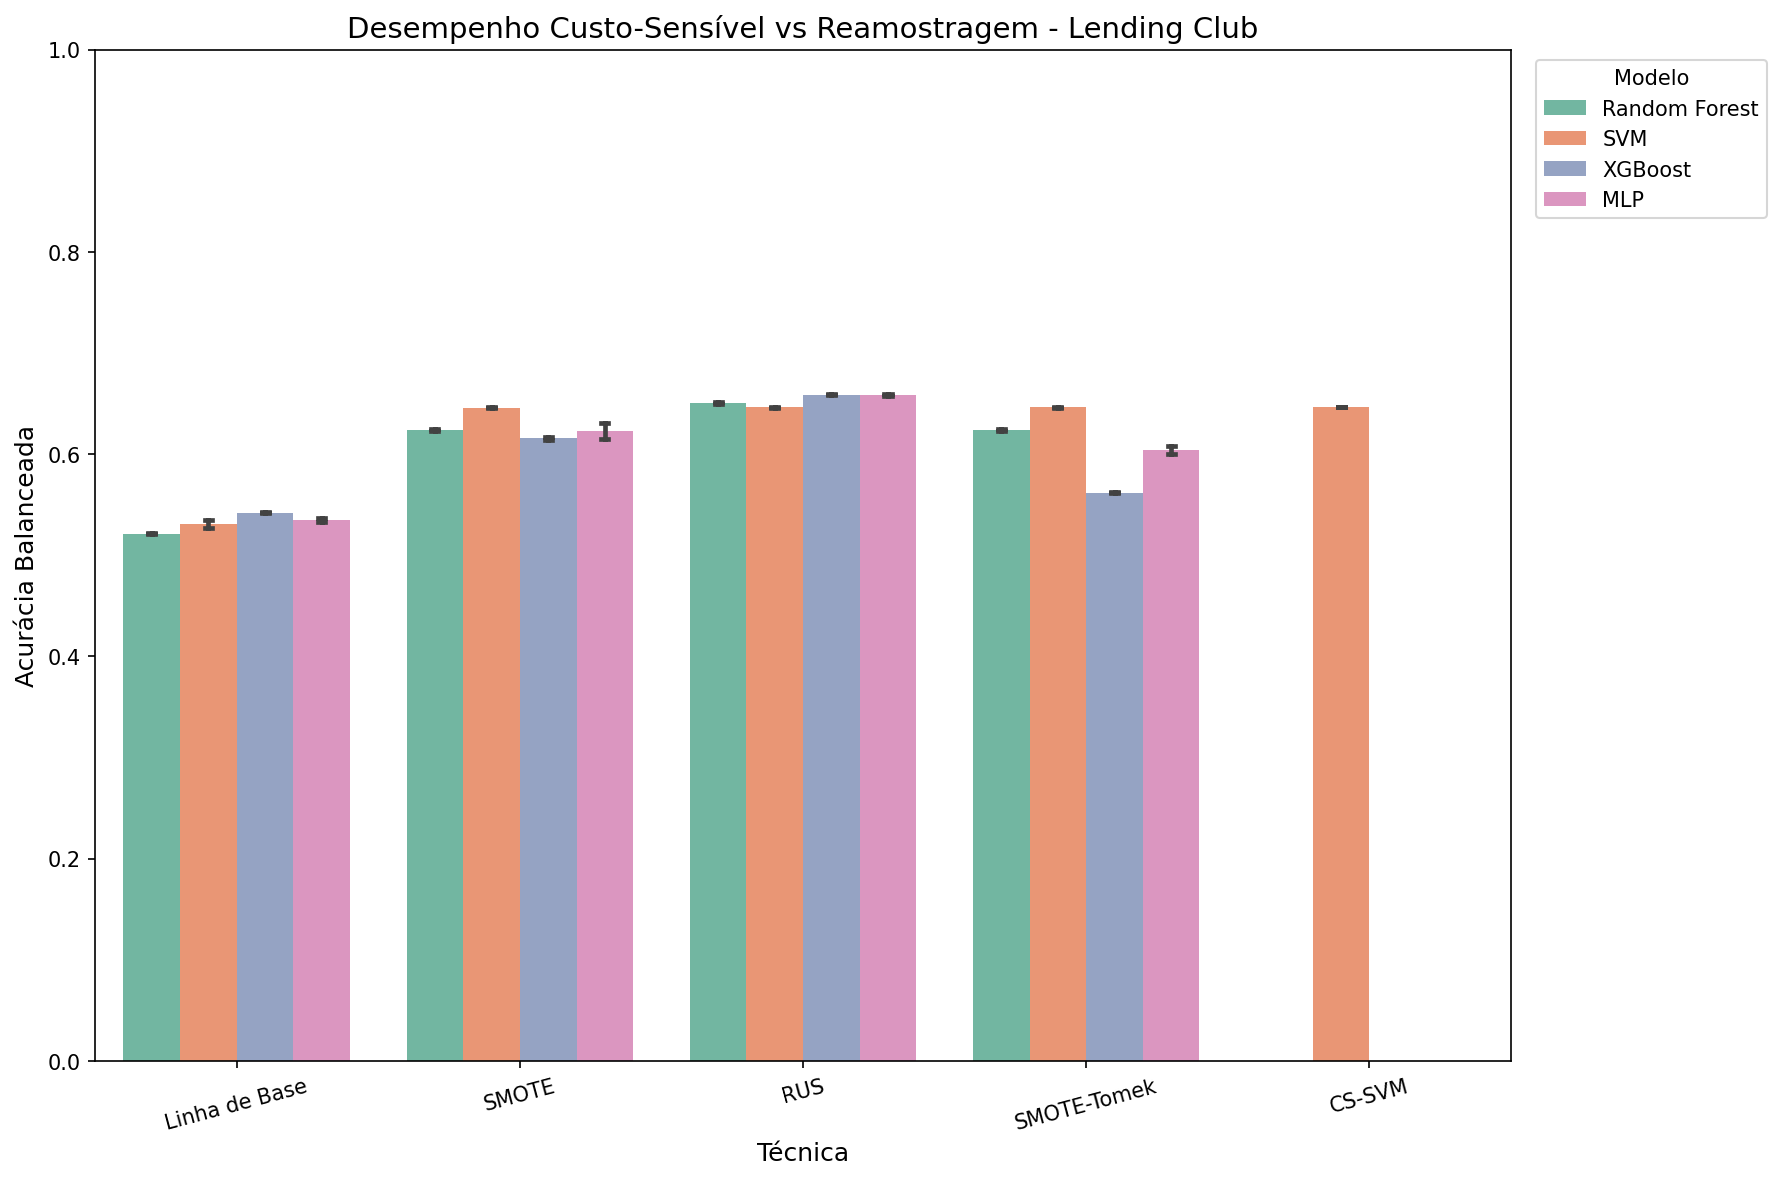
\includegraphics[width=0.92\textwidth,keepaspectratio]{experimentos/reports/pt_BR/lending_club/cs_vs_resampling_plot.png}
\end{frame}

\begin{frame}{Resultados}
  \vspace{-0.4em}
  \centering
  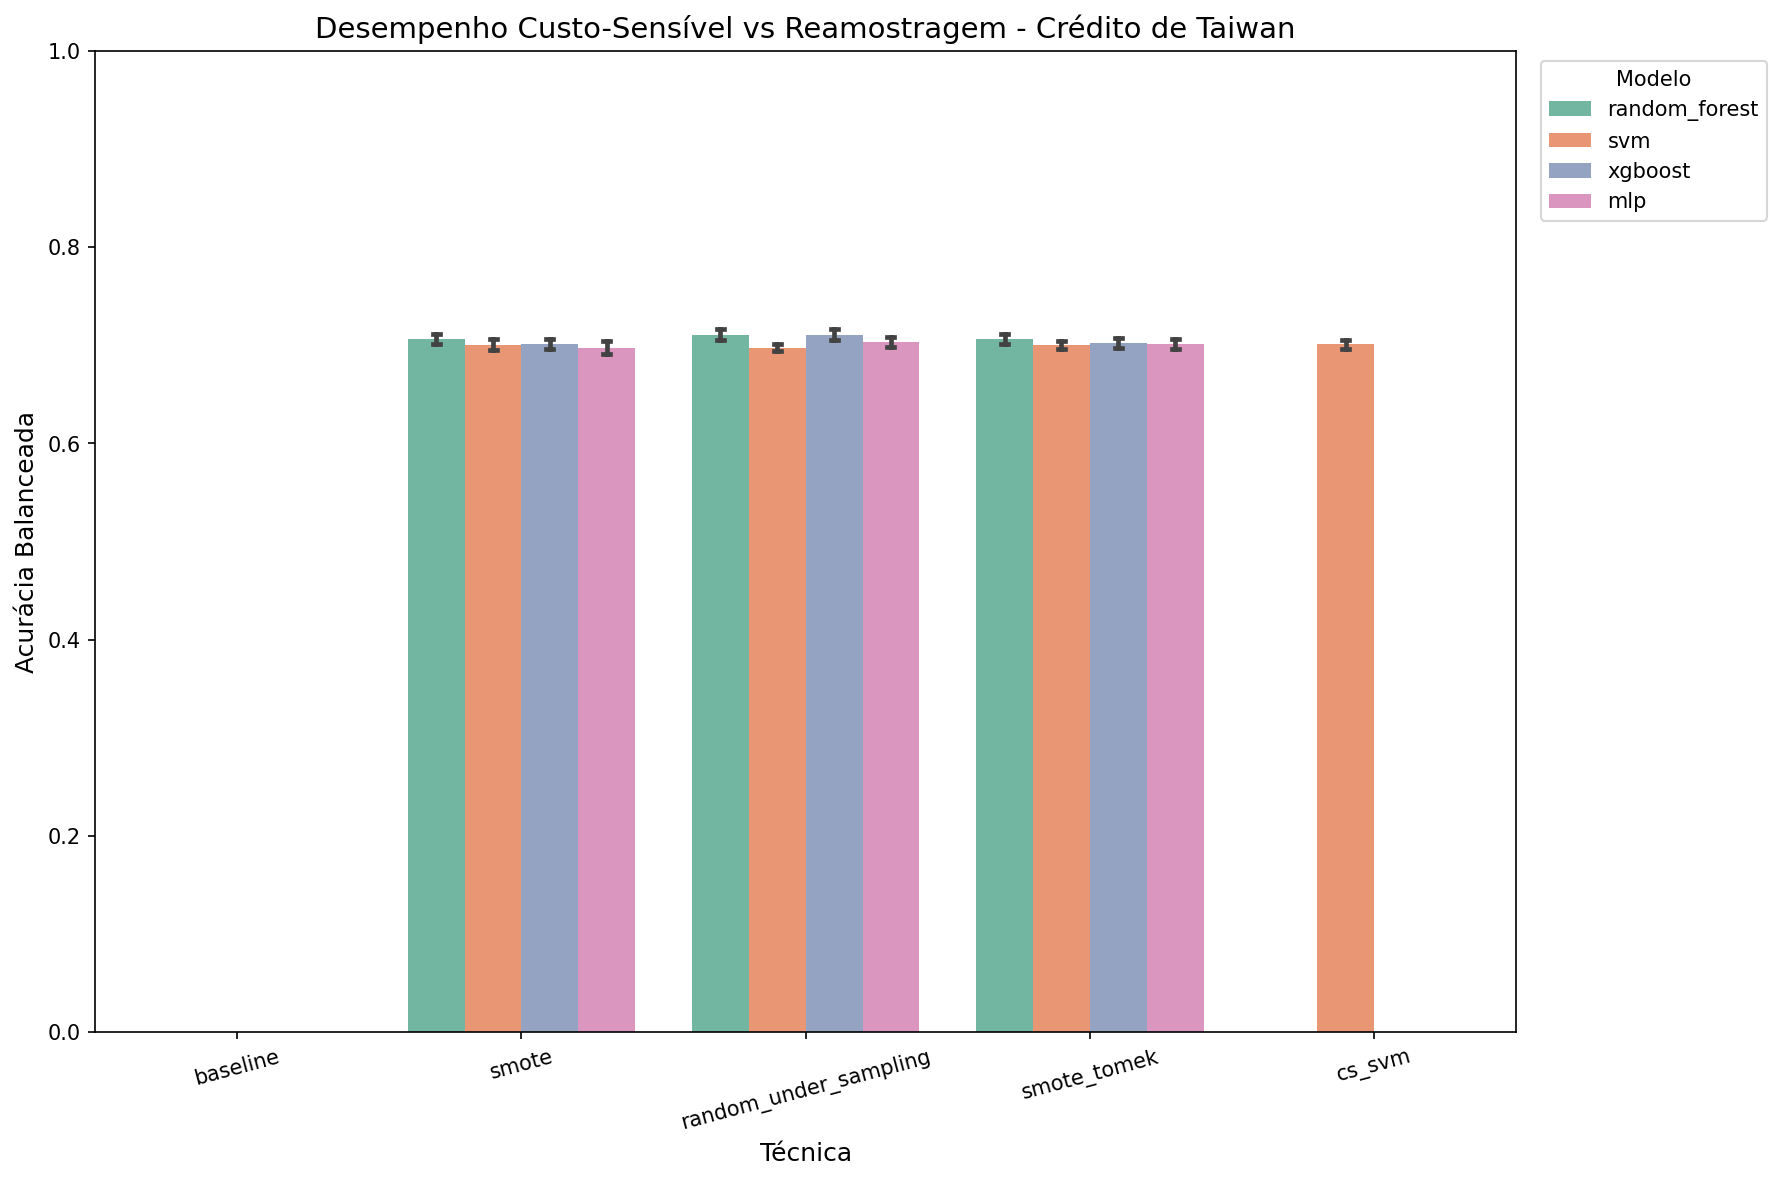
\includegraphics[width=0.92\textwidth,keepaspectratio]{experimentos/reports/pt_BR/taiwan_credit/cs_vs_resampling_plot.png}
\end{frame}

\begin{frame}{Resultados}
  \vspace{-0.4em}
  \centering
  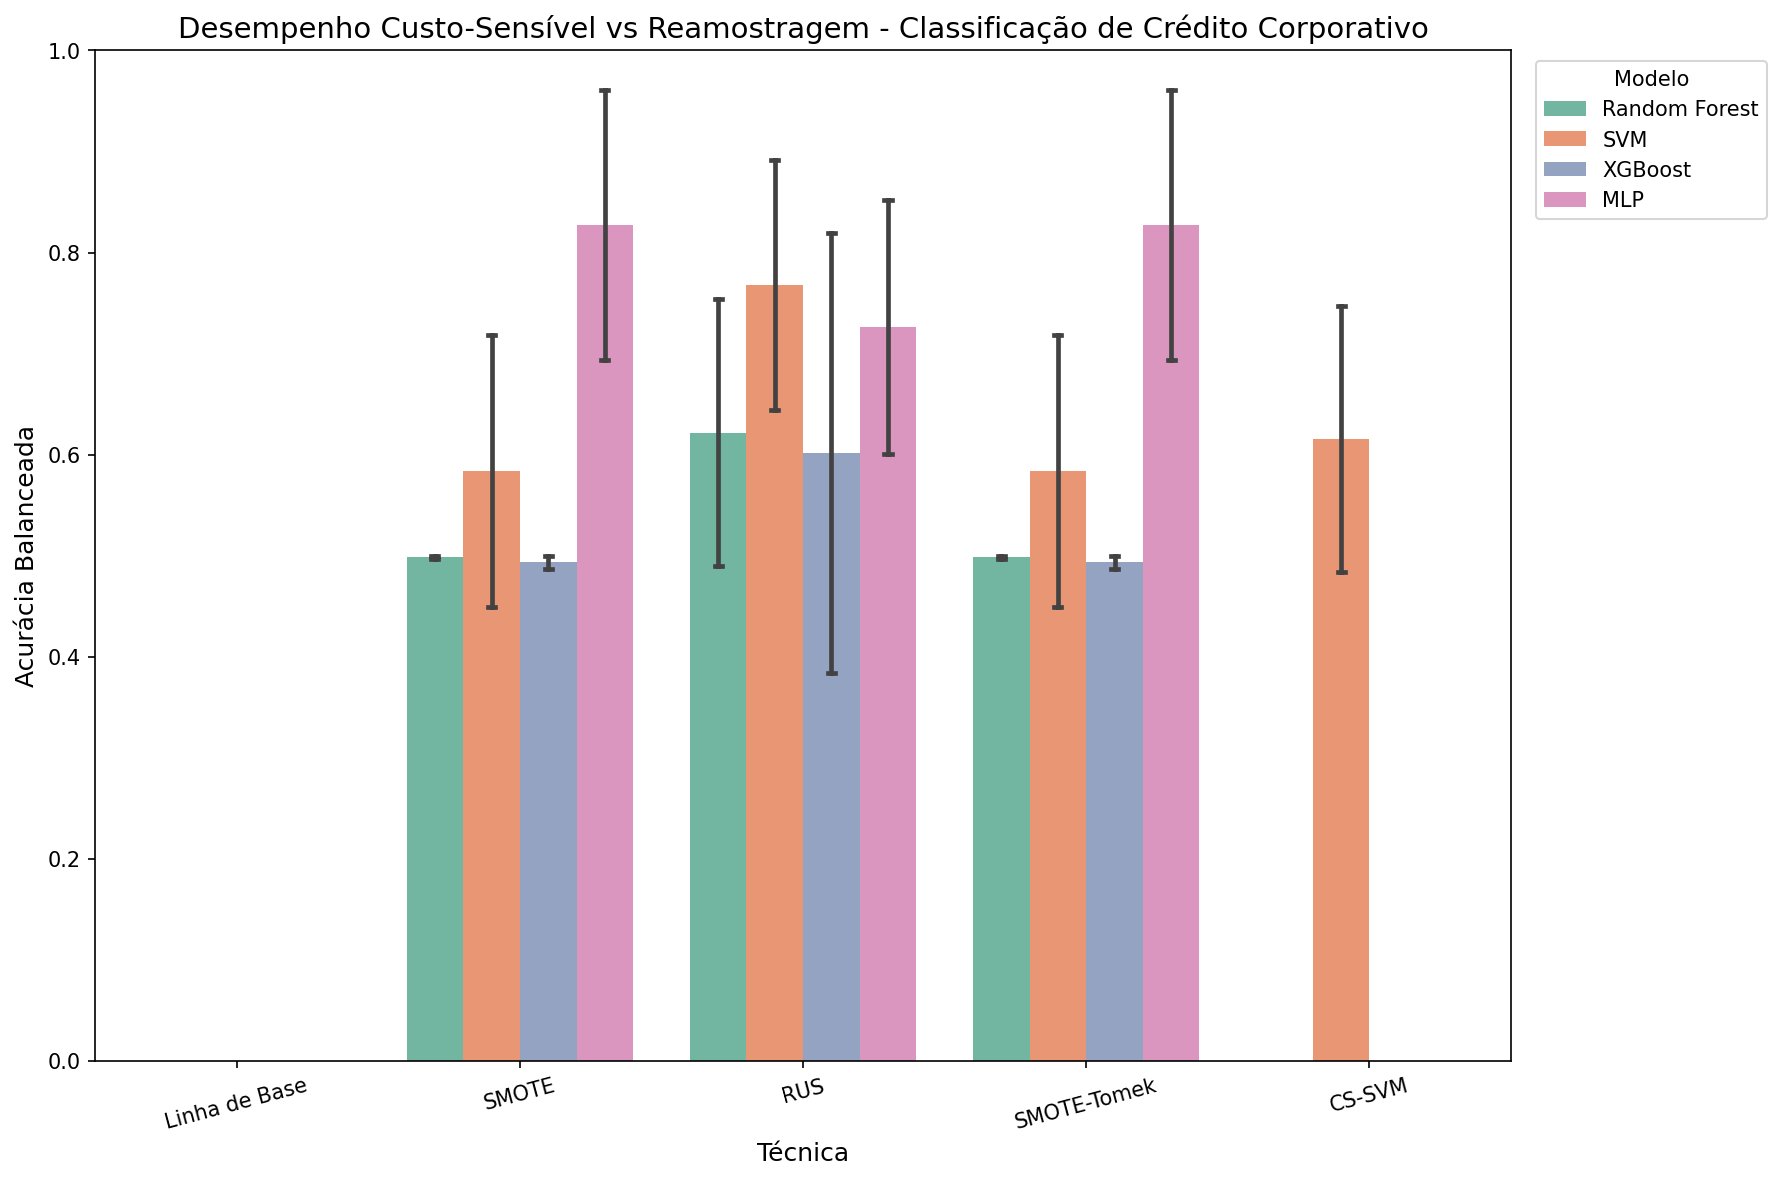
\includegraphics[width=0.92\textwidth,keepaspectratio]{experimentos/reports/pt_BR/corporate_credit_rating/cs_vs_resampling_plot.png}
\end{frame}

\begin{frame}{Resultados}
  \vspace{-0.4em}
  \centering
  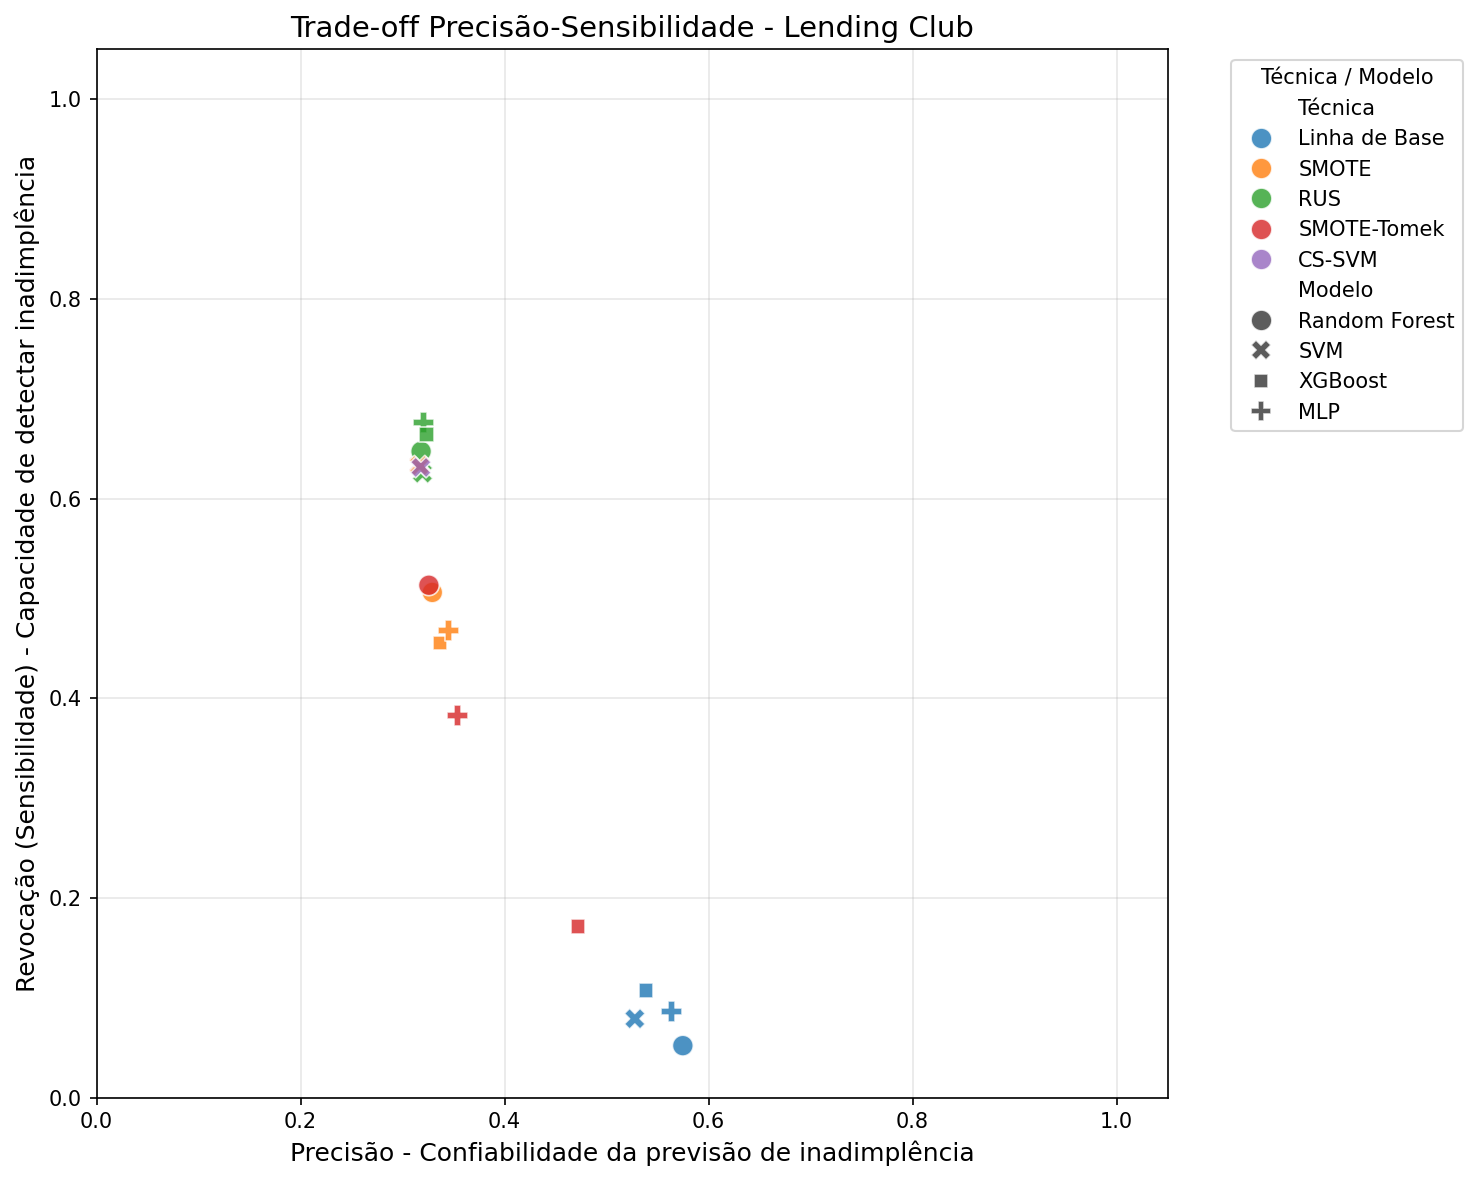
\includegraphics[width=0.90\textwidth,keepaspectratio]{experimentos/reports/pt_BR/lending_club/tradeoff_plot.png}
\end{frame}

\begin{frame}{Resultados}
  \vspace{-0.4em}
  \centering
  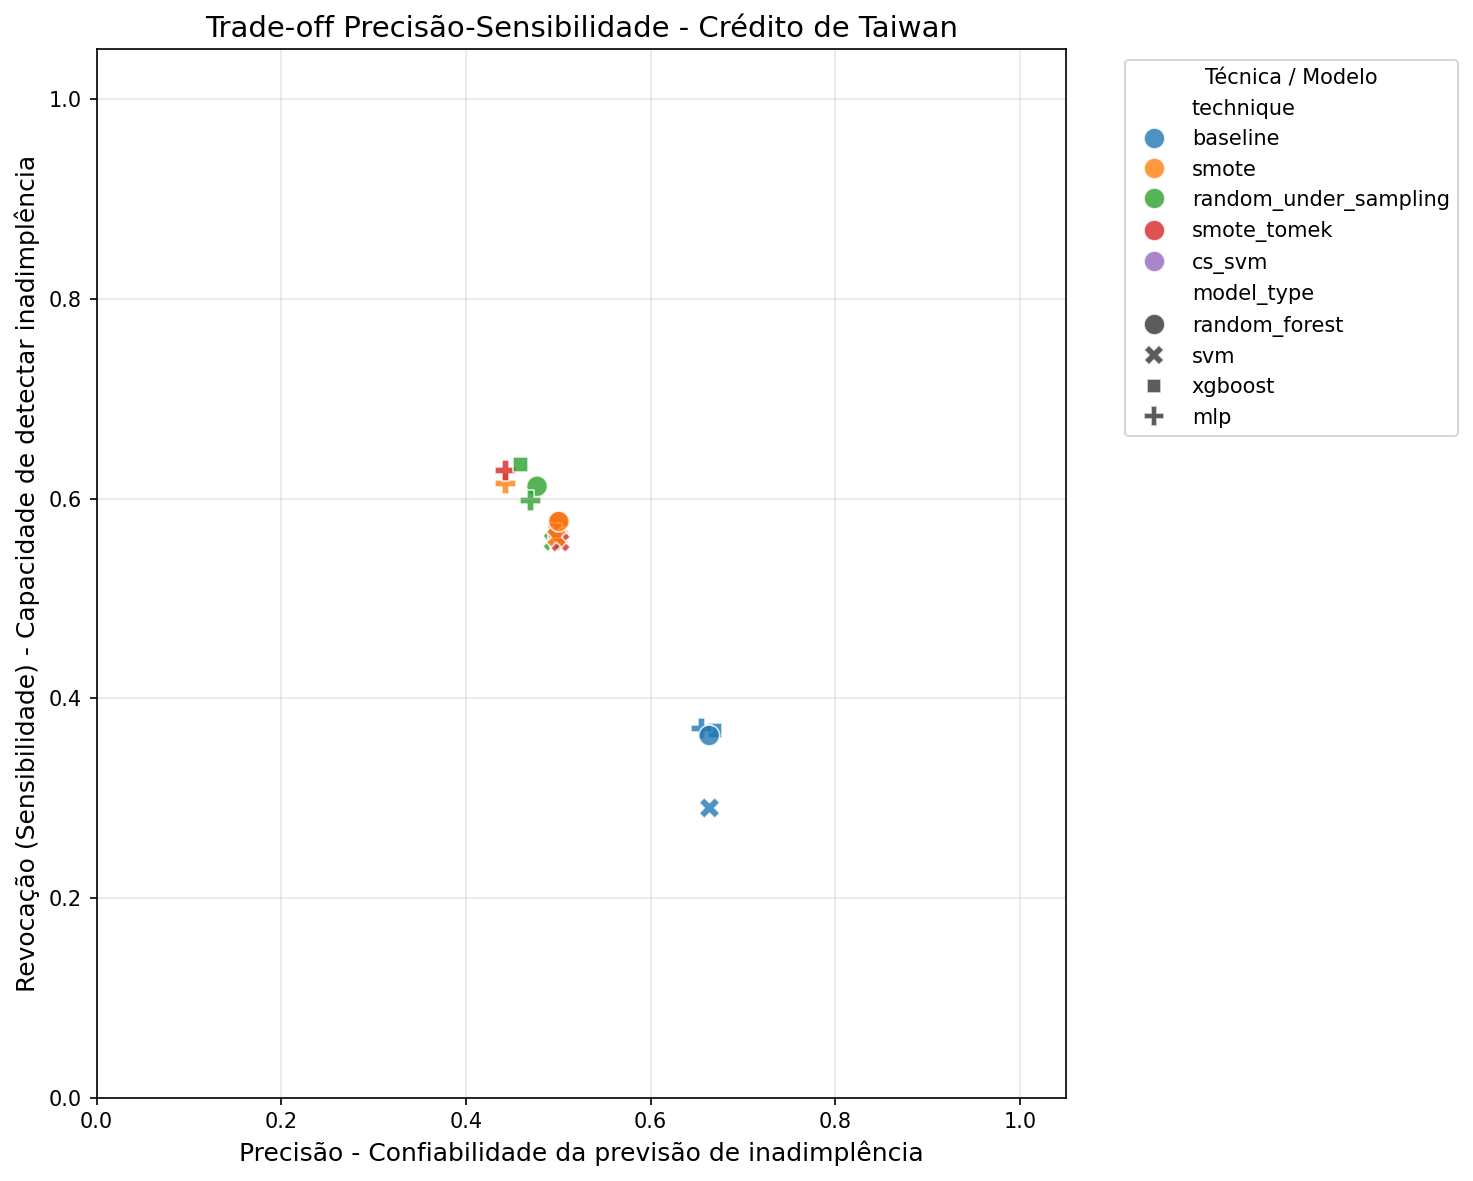
\includegraphics[width=0.90\textwidth,keepaspectratio]{experimentos/reports/pt_BR/taiwan_credit/tradeoff_plot.png}
\end{frame}

\begin{frame}{Resultados}
  \vspace{-0.4em}
  \centering
  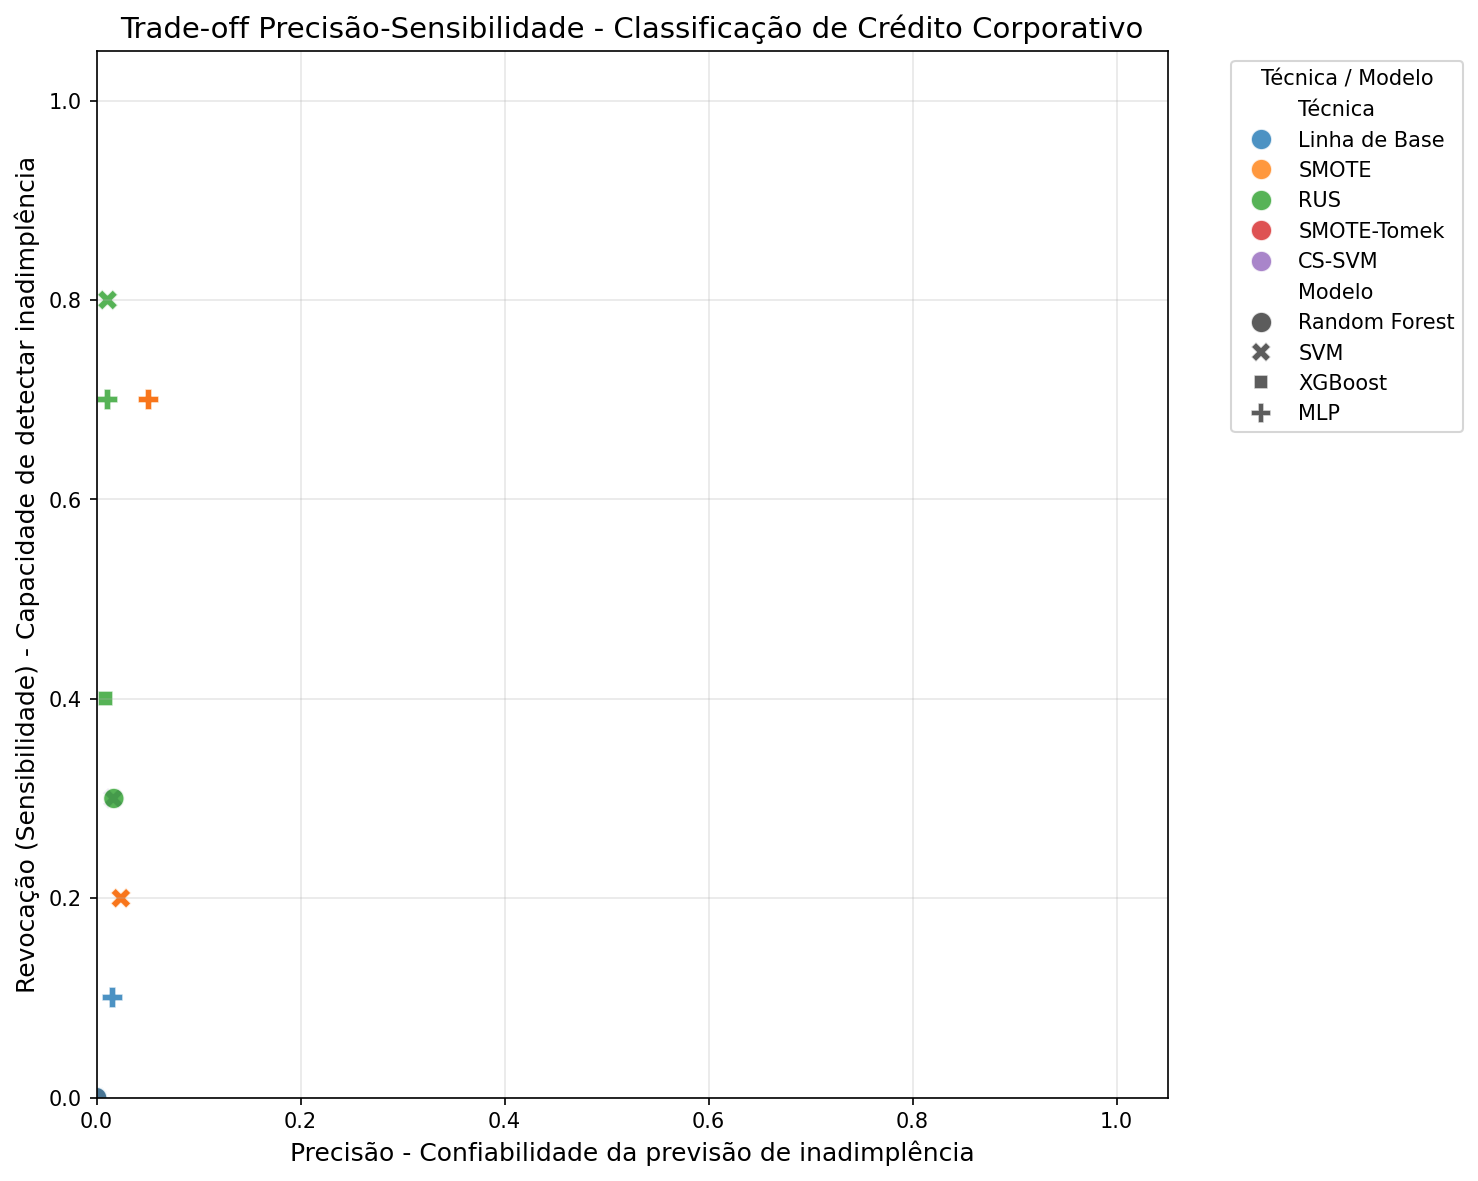
\includegraphics[width=0.90\textwidth,keepaspectratio]{experimentos/reports/pt_BR/corporate_credit_rating/tradeoff_plot.png}
\end{frame}

\begin{frame}{Discussão}
  \begin{itemize}
    \item[$\blacktriangleright$] Análise por contexto de crédito
      \begin{itemize}
        \item \textbf{Crédito Pessoal}
          \begin{itemize}
            \item Técnicas de re-amostragem, especialmente o RUS, apresentaram desempenho superior.
            \item Random Forest e XGBoost foram os modelos mais eficazes
          \end{itemize}
        \item \textbf{Crédito Corporativo}
          \begin{itemize}
            \item SMOTE se destacou como a técnica mais eficaz
            \item Desempenho geral foi baixo, devido ao pequeno número de amostras e à alta dimensionalidade dos dados.
          \end{itemize}
      \end{itemize}
  \end{itemize}
\end{frame}

\begin{frame}{Discussão}
  \begin{itemize}
    \item[$\blacktriangleright$] Desempenho Custo-sensível vs Re-amostragem
      \begin{itemize}
        \item Em geral, as estratégias de re-amostragem (RUS, SMOTE e SMOTE-Tomek) apresentaram desempenho superior em comparação com o CS-SVM.
        \item O CS-SVM mostrou-se competitivo em alguns casos, mas não conseguiu superar consistentemente as técnicas de re-amostragem.
      \end{itemize}
  \end{itemize}
\end{frame}

\begin{frame}{Discussão}
  \begin{itemize}
    \item[$\blacktriangleright$] \textit{Trade-off} entre Precisão e Sensibilidade
      \begin{itemize}
        \item As técnicas de re-amostragem, especialmente o RUS, tendem a melhorar a sensibilidade às classes minoritárias, mas isso pode ocorrer às custas da precisão.
        \item O CS-SVM apresentou um equilíbrio mais favorável entre precisão e sensibilidade em alguns casos, mas não foi suficiente para superar as técnicas de re-amostragem.
      \end{itemize}
  \end{itemize}
\end{frame}

\begin{frame}{Conclusão e trabalhos futuros}
  \begin{itemize}
    \item[$\blacktriangleright$] Conclusão
      \begin{itemize}
        \item As técnicas de re-amostragem mostraram-se eficazes para lidar com o desbalanceamento;
        \item Abordagens custo-sensíveis dependem fortemente da definição adequada dos custos de classificação;
        \item Não existe uma solução única para todos os contextos de crédito, e a escolha da técnica deve ser guiada pelas características específicas do conjunto de dados, como o grau de desbalanceamento, o número de amostras e a dimensionalidade dos dados.
      \end{itemize}
  \end{itemize}
\end{frame}

\begin{frame}{Conclusão e trabalhos futuros}
  \begin{itemize}
    \item[$\blacktriangleright$] Trabalhos futuros
      \begin{itemize}
        \item Explorar outras técnicas de re-amostragem, como o ADASYN e o SMOTE-ENN;
        \item Investigar a eficácia de técnicas de meta-aprendizado, como o MetaCost;
        \item Deep-Learning.
      \end{itemize}
  \end{itemize}
\end{frame}

\setbeamertemplate{bibliography item}{\insertbiblabel}
\setbeamercolor{bibliography item}{fg=black}
\setbeamercolor{bibliography entry author}{fg=black}
\setbeamercolor{bibliography entry title}{fg=black}
\setbeamercolor{bibliography entry location}{fg=black}
\setbeamercolor{bibliography entry note}{fg=black}

\begin{frame}[allowframebreaks, plain]{Referências}
  \bibliographystyle{plain}
  \bibliography{bibliografia}
\end{frame}
\end{document}